\documentclass[12pt, a4paper]{article}

\usepackage[utf8]{inputenc}
\usepackage[hmargin=2.5cm,vmargin=2.5cm]{geometry}
\usepackage[brazil]{babel}
\usepackage{graphicx}
\usepackage{amsmath}
\usepackage{steinmetz}
\usepackage{float}
\usepackage{graphicx}

\title{Relatório 1\\Exercício Prático \textit{PSpice}}
\author{Gustavo Ciotto Pinton - 117136}
\date{Abril 2013}

\begin{document}

    {\large
    \centerline{Exercício Prático 3}\\
    \centerline{Gustavo Ciotto Pinton 117136}
    }
    \section*{Questões}
    
    \begin{enumerate}
    
        \item Neste item, utiliza-se um transistor do tipo NMOS para simular o seu funcionamento nas regiões de triodo e saturação. O circuito utilizado para essa tarefa está representado na figura~\ref{circ31}, na seção \textbf{Anexos}. \\
        Os parâmetros configurados, conforme enunciado, foram \(V_t = 1.136 V\), \(W = 100 \mu m\), \(L = 10 \mu m\), \(k'_n = 100 \mu A/V^2\) e \(V_A = 100V\).
        
            
        Antes de qualquer análise sobre os gráficos gerados, é necessário saber como um transistor funciona. Este componente eletrônico pode operar em duas possíveis regiões (triodo ou saturação), caso a tensão entre os pinos da porta e fonte (\(V_{GS}\)) seja maior que uma tensão determinada pelo fabricante (\(V_t\)). Se o transistor estiver operando na região de saturação, então deve obedecer à expressão~\ref{eq: cond_sat}, e, caso contrário, está na região de triodo.
        
        \begin{equation} \label{eq: cond_sat}
            V_{DS} \geq V_{GS} - V_t \leftrightarrow V_D \geq V_{G} - V_t \leftrightarrow V_{DG} \geq - V_t
        \end{equation}
        
        Supondo região de saturação, a corrente que passa pelo transistor é dada pela equação~\ref{eq:c_sat}.
        
        \begin{equation} \label{eq:c_sat}
            I_{D} = \frac{1}{2}k'_n\frac{W}{L} (V_{GS} - V_t)^2
        \end{equation}
        
        Na região de triodo, a corrente é dada por \ref{eq:c_tri}.
        
        \begin{equation} \label{eq:c_tri}
            I_{D} = k'_n\frac{W}{L} \left [(V_{GS} - V_t)V_{DS} - \frac{1}{2}V_{DS}^2 \right]
        \end{equation}
        
       Conhecendo estas relações, pode-se calcular alguns valores importantes como a tensão mínima para que o NMOS opere na região de saturação e a sua corrente. De acordo com as equações \ref{eq: cond_sat} e \ref{eq:c_sat}, obtém-se a tabela abaixo:
       
            \begin{table} [h!]
            \caption{Tensões e correntes de saturação para valores de \(V_{GS}\). } \\
            \centering
            \label{table:tab_valores}
            
                \begin{tabular}{ c | c | c } 

                \(V_{GS}\) [V] & \(V_{DSmin} = V_{GS} - V_t\) [V] & \(I_{Dsat}\) [ \(\mu A\) ] \\
                \hline
                1.136 & 0 & 0 \\
                1.636 & 0.5 & 125 \\
                2.136 & 1.0 & 500 \\
                2.636 & 1.5 & 1125\\
                3.136 & 2.0 & 2000\\
                
                \end{tabular}
           \end{table}   
       
       Os gráficos, um para cada valor de \(V_{GS}\) da tabela, obtidos pela simulação estão representados na figura \ref{graf31} na seção \textbf{Anexos}. As regiões de saturação são aquelas que se iniciam nas tensões \(V_{DSmin}\), presentes na segunda coluna da tabela, cada qual com sua respectiva corrente que, teoricamente, nunca muda para quaisquer valores maiores que estas tensões. Em outras palavras, pela teoria, a partir destes valores, os gráficos deveriam apresentar uma natureza linear, mais especificamente linhas paralelas à horizontal. Na figura \ref{graf31}, o que se vê na prática são retas muito próximas da horizontal. Em relação aos valores \(V_{DSmin}\) encontrados na tabela, embora muito próximos, eles não correspondem exatamente aos pontos em que as regiões de saturação iniciam. Uma das possíveis causas para essas diferenças entre a teoria e prática seria o fato de que nos cálculos não foi considerado o \textit{efeito Early}, ao contrário do que o software SPICE fez.
       
       Obviamente, as regiões de triodo são aquelas em que os valores das tensões \(V_{DS}\) são menores que os \(V_{DSmin}\) da tabela \ref{table:tab_valores} e que seguem a equação \ref{eq:c_tri}, isto é, possuem um caráter parabolóico. Como esperado, as curvas obtidas nestes intervalos na figura \ref{graf31} são realmente parábolas.
       
       \item Tomando os valores \(C_{C1} = C_{C2} = C_{S} = 100nF\), \(R_L = 100k\Omega \), \(R_{sig} = 100\Omega \), \(I_D = 1.136 mA \), \(V_{D} = 4V \) e \(V_{DD} = -V_{SS} = 10V\), é possível calcular as tensões \(R_G\) e \(R_D\) através da análise do circuito. 
       
       Para se obter o valor de \(R_D\), utiliza-se a expressão \ref{eq:eq_vd}:
       
       \begin{equation} \label{eq:eq_vd}
       R_D = \frac{V_{DD}-V_D}{I_D}       
       \end{equation}
       
       O valor obtido é \(R_D = 5.281k\Omega \)
       
       
       
       Por efeito de análise, a tensão no pino da fonte \(V_S\) pode ser obitdo a partir da equação \ref{eq:c_sat}, supondo que o transistor opere no estado de saturação e sabendo os valores da corrente e de \(V_t\), chegando a:
       
       \begin{equation}
       V_{GS} = V_G - V_S = V_t + \sqrt{\frac{2I_D}{k_n'\frac{W}{L}}} 
        \end{equation}
       
       Utilizando os dados do transistor do item anterior ( \(V_t = 1.136 V\), \(W = 100 \mu m\), \(L = 10 \mu m\), \(k'_n = 100 \mu A/V^2\) e, por efeito de simplificação, \(V_A = 0\) ) e levando em conta que \(V_G = 0\), calcula-se \(V_S = -2.6433V\). Pode ser verificado através de \ref{eq: cond_sat} que, de fato, o transistor está saturado.
       
       
       Vimos durante as aulas que a resistência de \(R_G\) pode ser estimada de forma que seja da ordem de \textit{megaohms}. Uma quantia razoável para essa componente seria \(R_G = 10M\Omega \). 
       
       Finalmente, o circuito proveniente destes dados é mostrado na figura \ref{circ32}, na seção anexos.
       
       Fazendo uma simulação no SPICE por BIAS POINT DETAIL, obtém-se as tabelas \ref{table:tabelaBIAS} e \ref{table:tabelacorrenteBIAS}, cujos dados foram retirados de um trecho do \textit{output file} gerado pela simulação.
       
       
        \begin{table} [h!]
            \caption{SMALL SIGNAL BIAS SOLUTION. } \\
            \centering
            \label{table:tabelaBIAS}
            
                \begin{tabular}{ c | c | c | c } 
        
                NODE & VOLTAGE & NODE & VOLTAGE \\
                \hline
                C_{C1} & 0.0000 & R_G & 0.0000 \\
                R_{sig} & 0.0000 & V_{DD} & 10.0000 \\
                V_{SS} & -10.0000 & C_S & -2.6433\\
                C_{C2} & 4.0008 & R_L & 0.0000 \\
                
                \end{tabular}
       \end{table}   
             
    
        \begin{table} [h!]
            \caption{VOLTAGE SOURCE CURRENTS. } \\
            \centering
            \label{table:tabelacorrenteBIAS}
            
                \begin{tabular}{ c | c} 
        
                NAME & CURRENT\\
                \hline
                V_{sig} & 0.000E+00 \\
                V_{DD} & -1.136E-03  \\
                V_{SS} & -1.136E-03
                
                \end{tabular}
       \end{table} 

       É possível verificar que todos as tensões da tabela \ref{table:tabelaBIAS} correspondem exatamente a aqueles calculados pela teoria, exceto a voltagem em \(C_{C2}\) (ou \(V_D\)) que deveria ser 4V. Essa pequena diferença de 0.0008 ocorreu devido a aproximação de casas decimais realizada na conta da resistência \(R_D\).
       
       Vamos analisar agora a função de transferência do circuito \ref{circ32}. Pode-se considerar que para altas frequências, os capacitores atuam como curto-circuito. Utilizando o modelo \(\pi \) para pequenos sinais, a tensão \(v_{gs}\) é dada pela equação \ref{eq:vgs}:
       
       \begin{equation} \label{eq:vgs}
       v_{in} = v_{gs} = \frac{R_G}{R_G+R_{sig}} v_{sig}
       \end{equation}
       
       A tensão de saída, por sua vez, é:
       
       \begin{equation} \label{eq:vout}
       v_{out} = -g_m\frac{R_L R_D}{R_L+R_D} v_{gs}
       \end{equation}
       
       Combinando \ref{eq:vgs} e \ref{eq:vout}, tem-se:
       
       \begin{equation} \label{eq:am}
       A_m = \frac{v_{out}}{v_{sig}} = -g_m\frac{R_L R_D}{R_L+R_D} \frac{R_G}{R_G+R_{sig}} 
       \end{equation}
    
        Para calcular \(g_m\), utiliza-se:
    
        \begin{equation} \label{eq:gm}
            g_{m} = k'_n\frac{W}{L} (V_{GS} - V_t)
        \end{equation}
    
        Sabendo que \(V_{GS} = V_G - V_S = 0 - (-2.6433) = 2.6433 V\) e \(V_t = 1.136V\), obtem-se \(g_m = 1.507 \frac{mA}{V}\). Finalmente, substituindo todos os valores em \ref{eq:am}, obtem-se \(A_m = -7.5592 \frac{V}{V}\).
        
        A figura \ref{graf32} da seção \textbf{Anexos} é um gráfico de \(\left|\frac{v_{out}}{v_{sig}}\right|\) pela frequência, ou seja, um gráfico que representa \(\left|A_m|\right\). Portanto, o valor desta função para grandes frequências deveria, teoricamente, permanecer em 7.5592. 
        
        Olhando atentamente para a figura, nota-se facilmente que é exatamente isto o que ocorre, isto é, a transferência, para grandes frequências, é muito próxima ao valor de \(\left|A_m\right| = 7.5592 \), com um erro relativo estimado em aproximadamente 4\%.
    
    
    A função de corte para baixas, \(f_L\), considerando que \(C_S\) é o capacitor que interfere mais significantemente neste valor, é dada pela expressão:
    
    \begin{equation}
    f_L = \frac{g_m}{2\pi C_S}    
    \end{equation}
    
    Substuindo os valores, chega-se a \(f_L = 2398.5 Hz\). Novamente, se olharmos no gráfico \ref{graf32} a frequência correspondente ao ganho \(\frac{7.5592}{2} = 3.7796\), veremos que o seu valor está muito próximo daquele que calculamos teoricamente (em erro relativo de aprox. 7\%).
    
    \item Vamos agora analisar o circuito de uma inversor lógico construído a partir de um transistor PMOS e um NMOS. O circuito que será analisado primeiramente está representado na figura \ref{circ331} na seção \textbf{Anexos}.
    
    A função de transferência entre as voltagens de entrada e saída está representada no gráfico da figura \ref{graf331}. Nele, destacam-se cinco regiões de condução dos transistores. Resumidamente:
    
        \begin{itemize}
            
            \item \textit{NMOS cortado e PMOS saturado}: A condição para que um NMOS conduza corrente é que \(V_{GS} \geq V_{tn} \), que é equivalente a dizer que \(V_{G} \geq V_{tn} \), uma vez que, neste caso, \(V_S = 0\). Esta condição claramente não será atendida no intervalo [0, \(V_{tn}\)) e o NMOS não conduzirá. Por outro lado, o PMOS estará conduzindo em condição saturada, já que, para toda tensão de entrada \(V_{SG} \geq V_{SG} - |V_t|\).
            
            \item \textit{NMOS triodo e PMOS saturado}: Após a condição de condução ser atendida, o NMOS pode estar operando em triodo ou em saturação. Para operar em saturação, a condição descrita pela equação \ref{eq: cond_sat} deve ser atendida. Isso claramente não ocorre até \(V_{in}\) atingir o valor de \(\frac{V_{CC}}{2}\).
            
            \item \textit{NMOS e PMOS saturados}: esta faixa de valores corresponde às tensões de entrada em ambas as condições de saturação são atendidas.
            
           \item \textit{NMOS saturado e PMOS triodo}: semelhante ao caso 2, guardadas as inversões.
            
            \item \textit{NMOS saturado e PMOS cortado}:  semelhante ao caso 1, guardadas as inversões.
        \end{itemize}
        
            \\
            Uma segunda maneira de ser visualizar estes estados é através do gráfico de transferência de corrente por tensão de entrada, ilustrado na figura \ref{graf332}. Através deste gráfico, é possível notar que, nas proximidades de t = 0, a corrente de bateria tende a 0. Isto ocorre porque até que \(V_{in}\) alcance \(V_t\), o NMOS permanece cortado e, deste modo, \(V_{CC} = V_o\), o que implica a inexistência de quaisquer correntes.
            \\
            
            Finalmente, vamos analisar o caso em que colocamos um capacitor na saída do inversor, gerando o circuito \ref{circ332}. A análise do transitório da saída deste circuito é dada pela figura \ref{graf334}, através de sua tensão, ou pela figura \ref{graf335}, através de sua corrente. Pelo gráfico \ref{graf334}, nota-se que nas regiões em que o sinal muda de alto para baixo ou vice-versa, há a presença de pequenas ondulações causadas pelo carregamento ou descarremento do capacitor.
            \\
            
            Sabe-se que \(i = \frac{dQ}{dt} \to idt = dQ \to \Delta Q = i \Delta t \). Sendo assim, a carga fornecida pela bateria pode ser calculada pela área do gráfico ilustrado em  \ref{graf335}. A área obtida foi aproximadamente \(Q_{area} \approx \frac{7.5mA * 1.8 \mu s}{2} \approx 6.75nC \). Por efeito de comparação, o valor teórico esperado é dado por \( Q = CV_{DD} = 5.68nC \). O erro relativo entre esses valores é de aproximadamente 19\% e pode ser perfeitamente explicado pela imprecisão no cálculo da área. 
            
            Por último, a energia que é fornecida pela bateria durante o carregamento do capacitor pode ser calculada por :
            
            \begin{equation}
            E = V_{DD}Q
            \end{equation}
            
            cujo resultado, para nossos dados, é \(E = 33.75nJ\). Novamente por efeito de comparação, o resultado esperado seria \(E = CV_{DD}^2 = 28.4nJ\) e o erro relativo obtido foi de aprox. 20\%, podendo ser explicado pelos meios do cálculo de \(Q_{area}\)
            
        \end{itemize}
    \end{enumerate}
    
    \newpage
    \section*{Anexos}
    
    \begin{figure}[h!] 
        \centering
        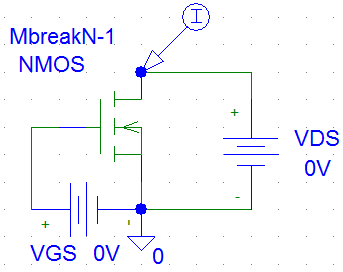
\includegraphics[width=0.4\textwidth]{circ31}
        \caption{Transitor NMOS.}        
        \label{circ31}
    \end{figure}
    
    \begin{figure}[h!] 
        \centering
        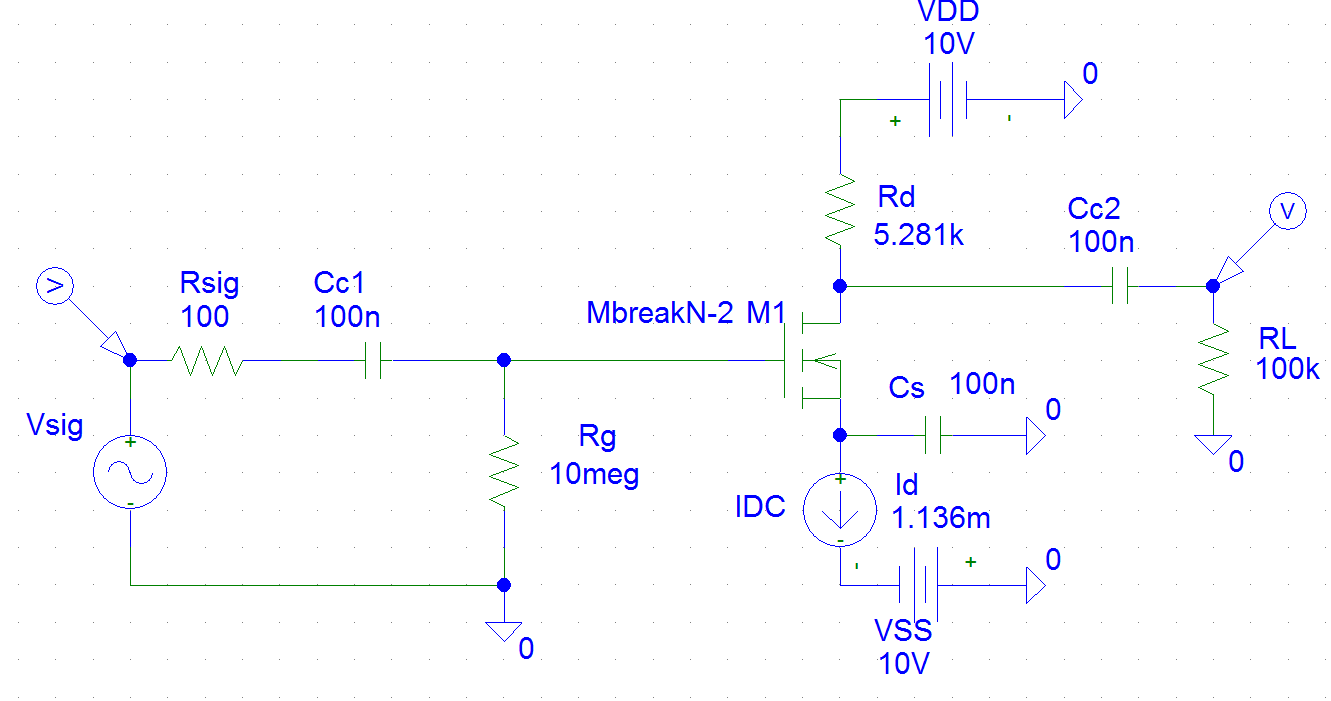
\includegraphics[width=1\textwidth]{circ32}
        \caption{Circuito NMOS polarizador de fonte comum.}        
        \label{circ32}
    \end{figure}
    
    \newpage
    
    \begin{figure}[h!] 
        \centering
        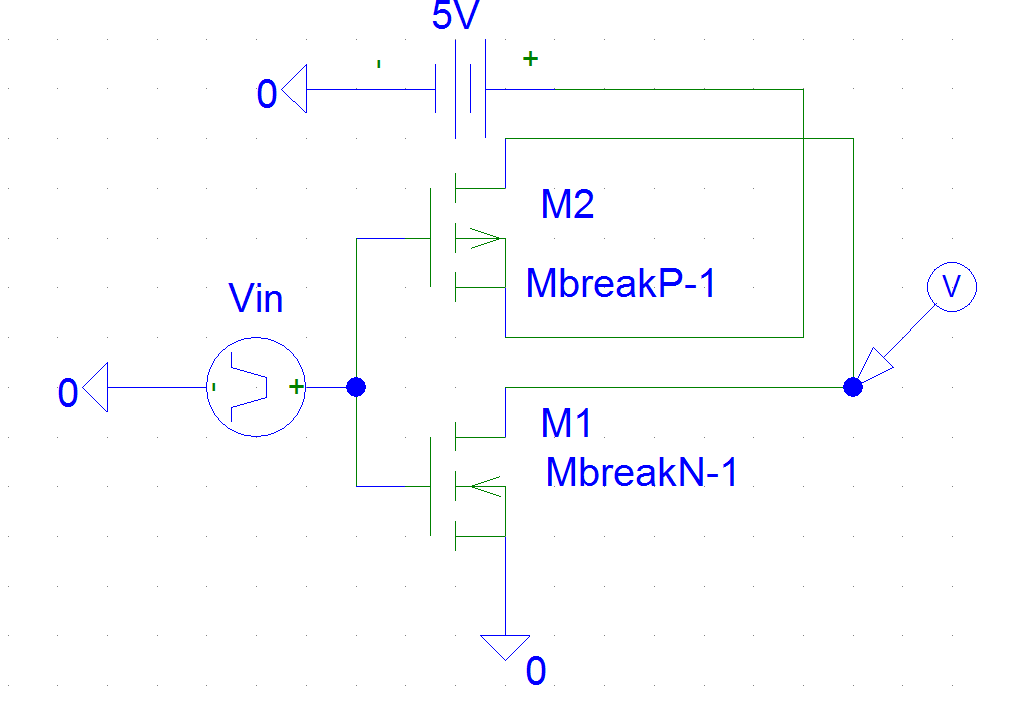
\includegraphics[width=0.6\textwidth]{circ331}
        \caption{Inversor CMOS.}        
        \label{circ331}
    \end{figure}
    
    \begin{figure}[h!] 
        \centering
        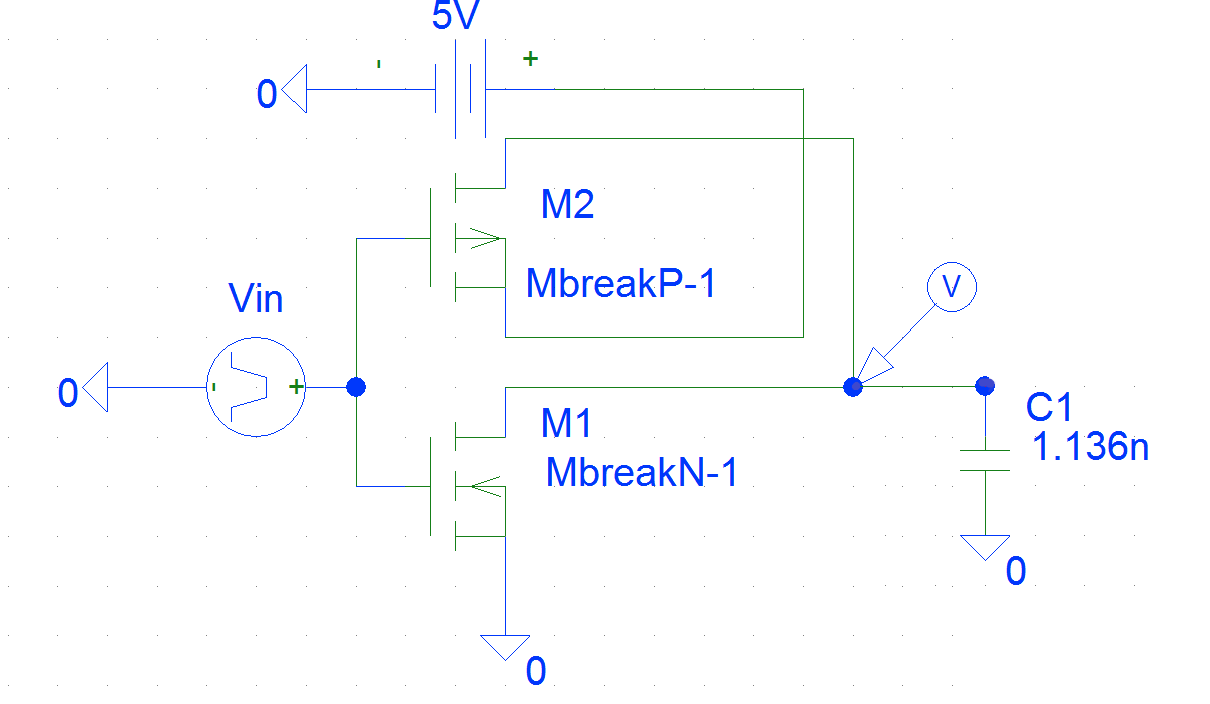
\includegraphics[width=0.8\textwidth]{circ332}
        \caption{Inversor CMOS com capacitâncias parasitas.}        
        \label{circ332}
    \end{figure}
    
    \newpage
    
    \begin{figure}[h!] 
        \centering
        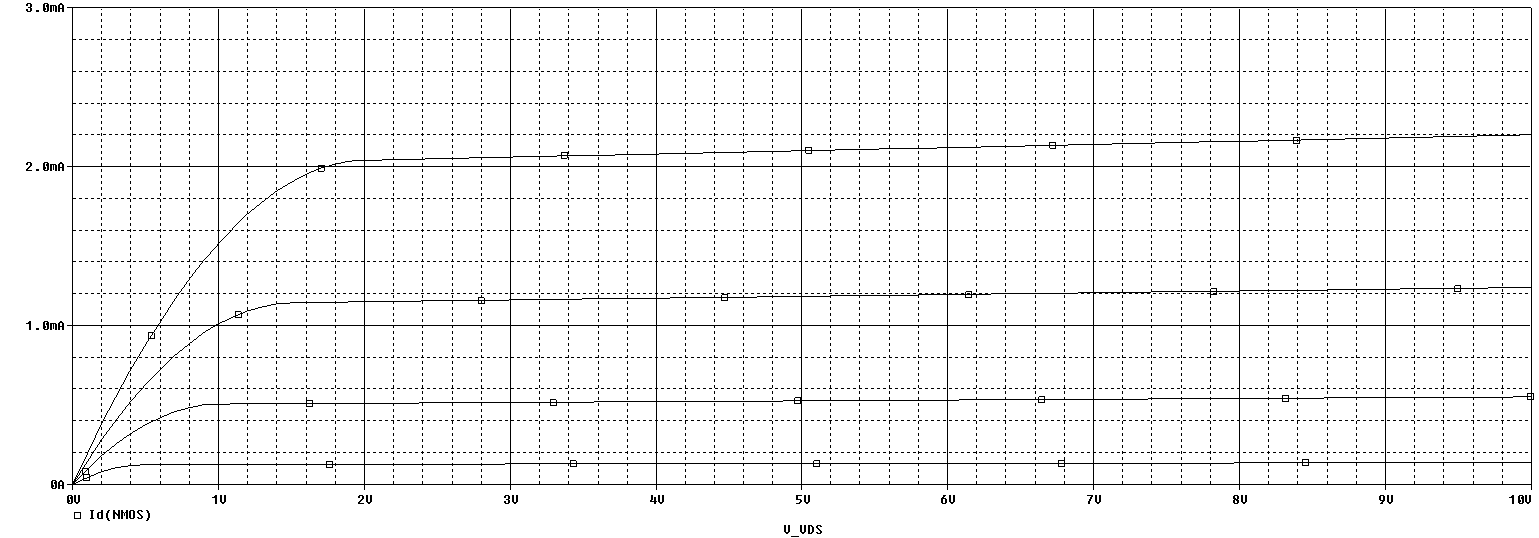
\includegraphics[width=1\textheight, angle=-90]{graf31}
        \caption{Curvas de corrente versus \(V_{DS}\).}        
        \label{graf31}
    \end{figure}
    
    \newpage
    
    \begin{figure}[h!] 
        \centering
        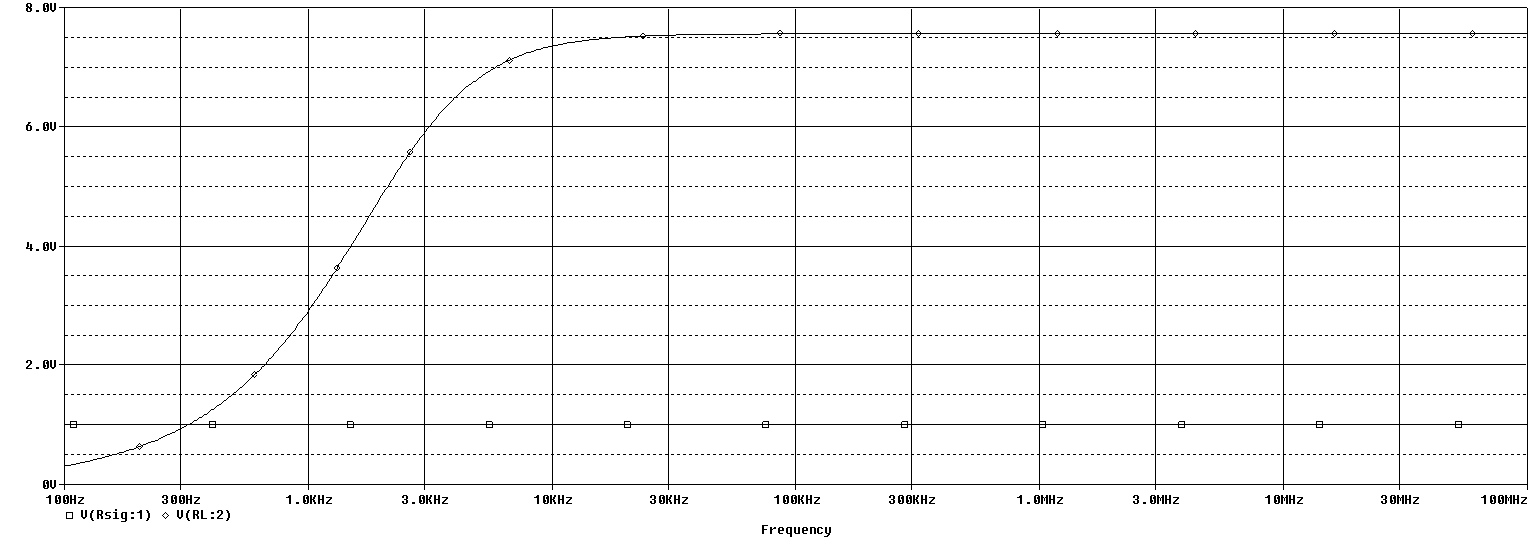
\includegraphics[width=1\textheight, angle=-90]{graf32}
        \caption{Função de transferência .}        
        \label{graf32}
    \end{figure}
    
    \newpage
    
    \begin{figure}[h!] 
        \centering
        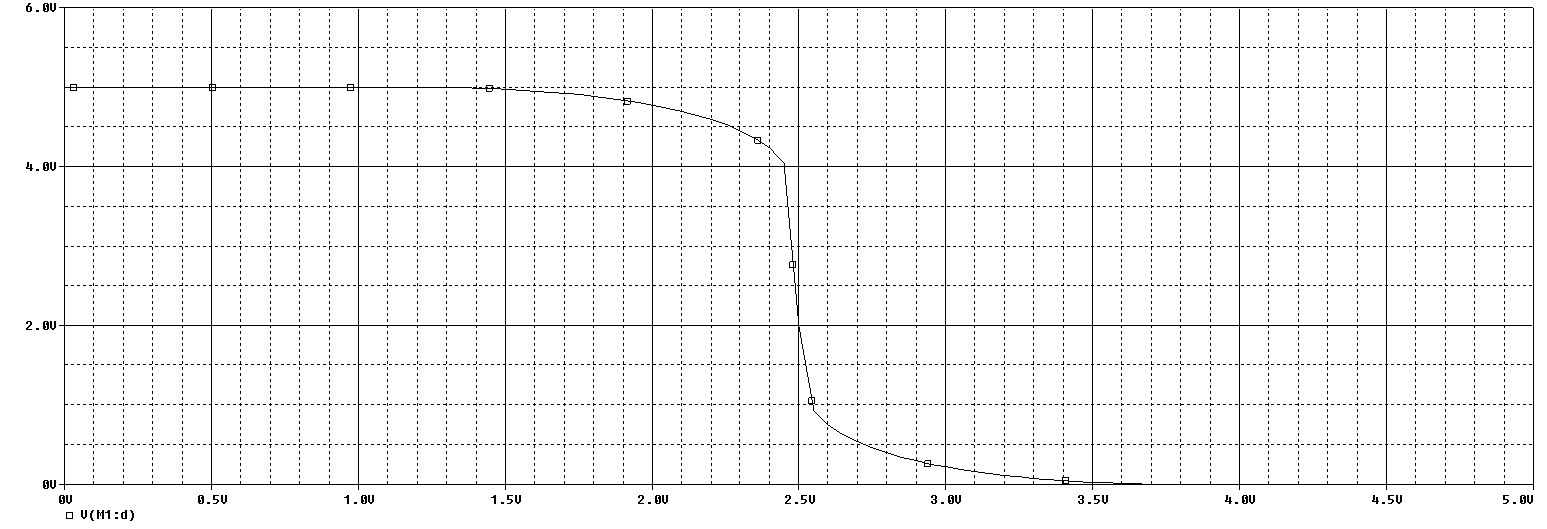
\includegraphics[width=1\textheight, angle=-90]{graf331}
        \caption{Função de transferência entre tensões de um inversor.}        
        \label{graf331}
    \end{figure}
    
    \newpage
    
    \begin{figure}[h!] 
        \centering
        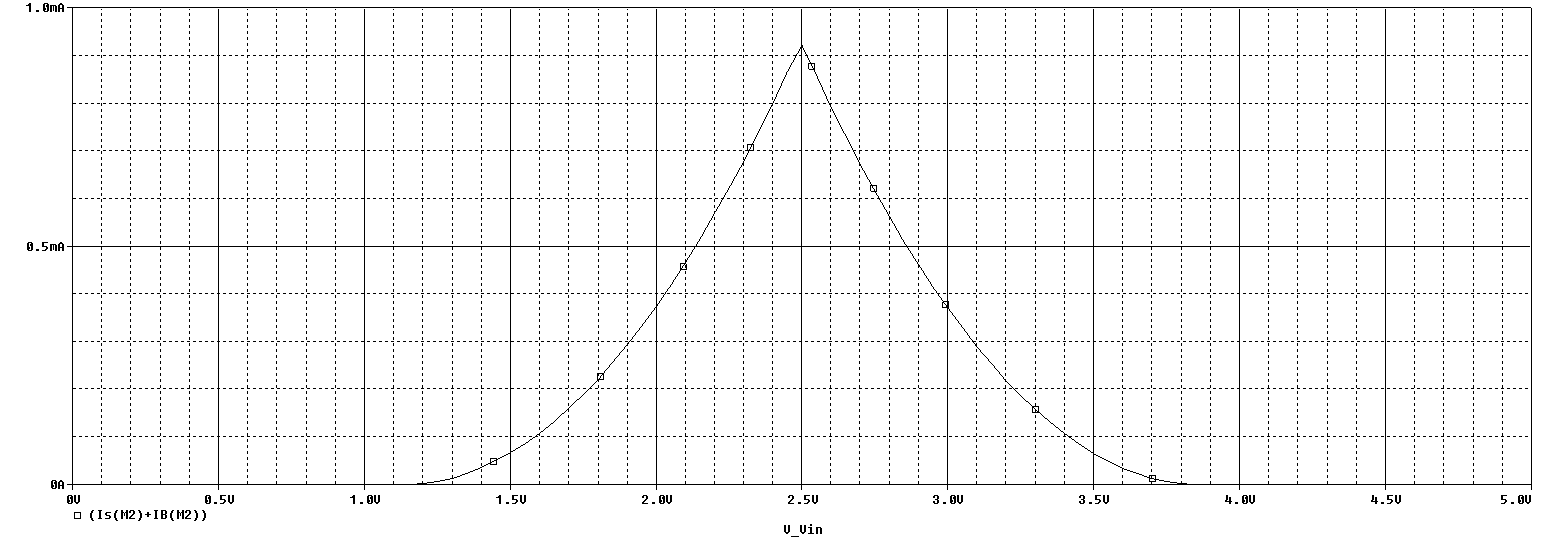
\includegraphics[width=1\textheight, angle=-90]{graf332}
        \caption{Função de transferência entre corrente e tensão de um inversor.}        
        \label{graf332}
    \end{figure}
    
    \newpage
    
    \begin{figure}[h!] 
        \centering
        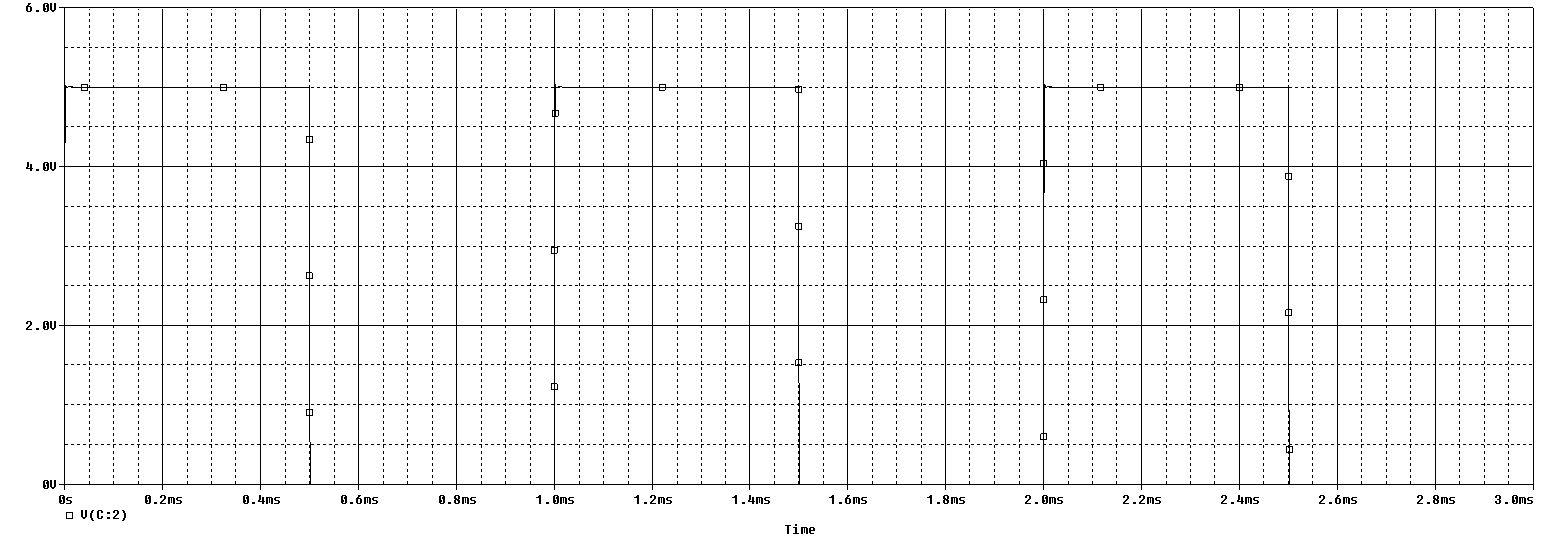
\includegraphics[width=1\textheight, angle=-90]{graf333}
        \caption{Análise do transitório da função de saída.}        
        \label{graf334}
    \end{figure}
    
    \newpage
    
    \begin{figure}[h!] 
        \centering
        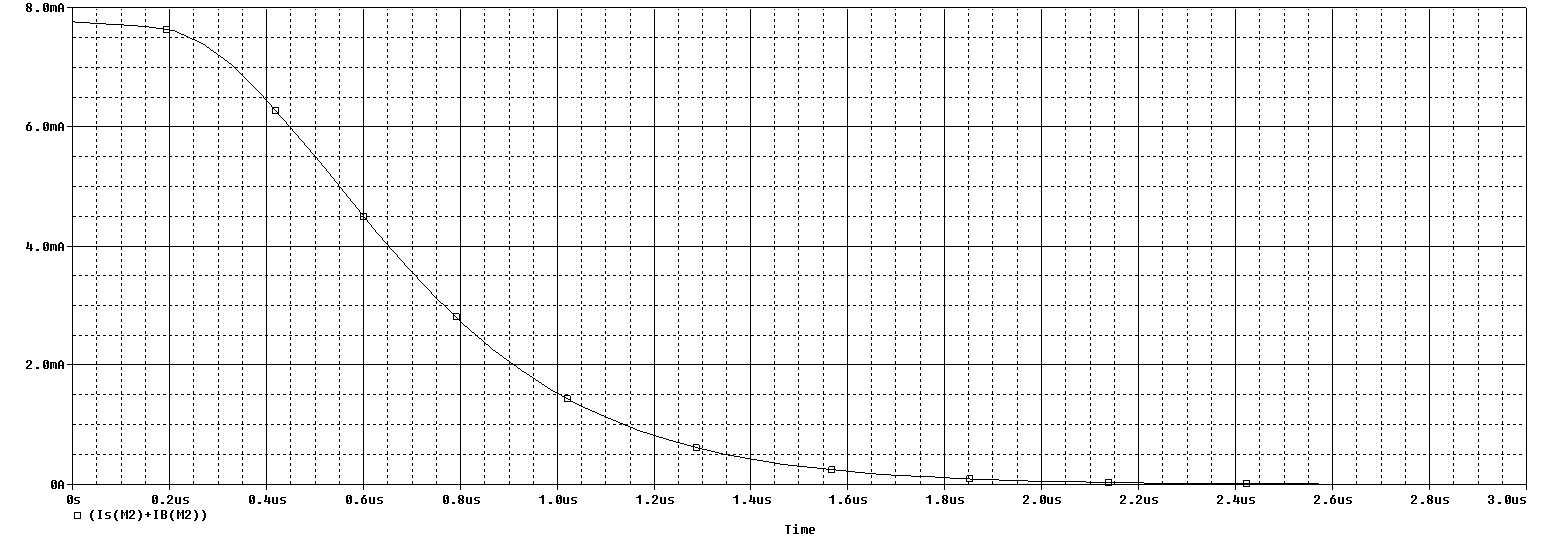
\includegraphics[width=1\textheight, angle=-90]{graf335}
        \caption{Análise da corrente na vizinhaça de t = 0.}        
        \label{graf335}
    \end{figure}
    
    
    
\end{document}